% Copyright 2020  Ed Bueler

\documentclass[10pt,hyperref]{beamer}

\mode<presentation>{
  \usetheme{Madrid}
  \usecolortheme{beaver}
  \setbeamercovered{transparent}
  \setbeamerfont{frametitle}{size=\large}
}

\setbeamercolor*{block title}{bg=red!10}
\setbeamercolor*{block body}{bg=red!5}

\usepackage[english]{babel}
\usepackage[latin1]{inputenc}
\usepackage{times}
\usepackage[T1]{fontenc}
% Or whatever. Note that the encoding and the font should match. If T1
% does not look nice, try deleting the line with the fontenc.

\usepackage{empheq}
\usepackage{xspace}
\usepackage{verbatim,fancyvrb}

%\usepackage[colorlinks=true]{hyperref}
\hypersetup{colorlinks}

% If you wish to uncover everything in a step-wise fashion, uncomment
% the following command: 
%\beamerdefaultoverlayspecification{<+->}

\newcommand{\bb}{\mathbf{b}}
\newcommand{\bc}{\mathbf{c}}
\newcommand{\br}{\mathbf{r}}
\newcommand{\bx}{\mathbf{x}}
\newcommand{\by}{\mathbf{y}}
\newcommand{\bv}{\mathbf{v}}
\newcommand{\bu}{\mathbf{u}}
\newcommand{\bw}{\mathbf{w}}

\newcommand{\grad}{\nabla}

\newcommand{\CC}{\mathbb{C}}
\newcommand{\RR}{\mathbb{R}}

\newcommand{\ddt}[1]{\ensuremath{\frac{\partial #1}{\partial t}}}
\newcommand{\ddx}[1]{\ensuremath{\frac{\partial #1}{\partial x}}}
\newcommand{\Matlab}{\textsc{Matlab}\xspace}
\newcommand{\Octave}{\textsc{Octave}\xspace}
\newcommand{\MO}{\Matlab}
\newcommand{\eps}{\epsilon}
\newcommand{\image}{\operatorname{im}}

\newcommand{\ds}{\displaystyle}

\newcommand{\ip}[2]{\left<#1,#2\right>}

\newcommand{\trefcolumn}[1]{\begin{bmatrix} \phantom{x} \\ #1 \\ \phantom{x} \end{bmatrix}}
\newcommand{\trefmatrixtwo}[2]{\left[\begin{array}{c|c|c} & & \\ #1 & \dots & #2 \\ & & \end{array}\right]}
\newcommand{\trefmatrixthree}[3]{\left[\begin{array}{c|c|c|c} & & & \\ #1 & #2 & \dots & #3 \\ & & & \end{array}\right]}
\newcommand{\trefmatrixgroups}[4]{\left[\begin{array}{c|c|c|c|c|c} & & & & & \\ #1 & \dots & #2 & #3 & \dots & #4 \\ & & & & & \end{array}\right]}

\newcommand{\blocktwo}[4]{\left[\begin{array}{c|c} #1 & #2 \\ \hline #3 & #4 \end{array}\right]}

\newcommand{\bqed}{{\color{blue}\qed}}

\newcommand{\exer}[2]{\medskip\noindent \textbf{#1.}\quad #2}

% I think I want this:
\AtBeginSection[]
{
  \begin{frame}<beamer>
    \frametitle{Outline}
    \tableofcontents[currentsection,hideallsubsections]
  \end{frame}
}

\title[Finite-dimensional spectral theory II]{Finite-dimensional spectral theory}

\subtitle{part II: understanding the spectrum (and singular values)}

\author{Ed Bueler}

\institute[MATH 617]{MATH 617 Functional Analysis}

\date{Spring 2020}

\begin{document}
\beamertemplatenavigationsymbolsempty


\begin{frame}
  \maketitle
\end{frame}


\begin{frame}{what happened in part I}

\begin{itemize}
\item see part I first: \quad \href{http://bueler.github.io/M617S20/slides1.pdf}{\texttt{bueler.github.io/M617S20/slides1.pdf}}
\item \emph{definition.} for a square matrix $A\in\CC^{n\times n}$, the \emph{spectrum} is the set
    $$\sigma(A)=\left\{\lambda\in\CC\,\big|\,Av=\lambda v \text{ for some }v\ne 0\right\}$$
\item we proved:
    \begin{itemize}
    \item[] $A = Q T Q^*$ \quad \emph{Schur decomposition} \quad for any $A \in \CC^{n\times n}$
    \item[] $A = Q \Lambda Q^*$ \quad \emph{spectral theorem} \quad for normal ($AA^*=A^*A$) matrices
    \end{itemize}
where $Q$ is unitary, $T$ is upper-triangular, and $\Lambda$ is diagonal
    \begin{itemize}
    \item[$\circ$] both decompositions ``reveal'' the spectrum (on the diagonal of $T$ and $\Lambda$)
    \item[$\circ$] the spectral theorem for matrices is sometimes called the \emph{principal axis decomposition} for quadratic forms
    \end{itemize}
\item we will extend the spectral theorem to $\infty$-dimensions
    \begin{itemize}
    \item[$\circ$] \dots but not the Schur decomposition
    \item[$\circ$] in $\infty$-dimensions we want to use unitary maps because such maps preserve both vector space and metric structure
    \end{itemize}
\end{itemize}
\end{frame}


%\begin{frame}{table of contents}
%\tableofcontents
%\end{frame}


\begin{frame}{important class: unitary matrices}

\begin{itemize}
\item before we get started \dots
\end{itemize}

\begin{definition}
$U \in \CC^{n\times n}$ is \emph{unitary} if $U^*U=I$
\end{definition}

\begin{lemma}
Consider $\CC^n$ as a inner product space with $\ip{v}{w}=v^*w$ and the $2$-norm $\|v\|_2 = \sqrt{\ip v v}$.  Suppose $U$ is linear map on $\CC^n$.  The following are equivalent:

\begin{itemize}
\item $U$ is unitary
\item expressed in the standard basis, the columns of $U$ are ON basis of $\CC^n$
\item $\ip{Uv}{Uw}=\ip{v}{w}$ for all $v\in\CC^n$
\item $\|Uv\|_2=\|v\|_2$ for all $v\in\CC^n$
\item $U$ is a metric-space isometry
\end{itemize}
\end{lemma}
\end{frame}


\begin{frame}{important class: normal matrices}

\begin{definition}
$A \in \CC^{n\times n}$ is \emph{normal} if $A^*A=AA^*$
\end{definition}

\begin{lemma}
Consider $\CC^n$ as a inner product space with $\ip{v}{w}=v^*w$ and the $2$-norm $\|v\|_2 = \sqrt{\ip v v}$.  Suppose $A$ is linear map on $\CC^n$.  The following are equivalent:

\begin{itemize}
\item $A$ is normal
\item $\|Ax\|_2 = \|A^*x\|_2$ for all $x$
\item exists an ON basis of eigenvectors of $A$
\item exists $Q$ unitary and $\Lambda$ diagonal so that $A=Q\Lambda Q^*$ (\emph{spectral theorem})
\end{itemize}
\end{lemma}
\end{frame}


\section{functional calculus}

\begin{frame}{power series of matrices}

\begin{itemize}
\item suppose $A$ is diagonalizable: $A = S \Lambda S^{-1}$
    \begin{itemize}
    \item[$\circ$] where $S$ is invertible and $\Lambda$ is diagonal
    \item[$\circ$] diagonal entries of $\Lambda$ are eigenvalues of $A$: $A v_i = \Lambda_{ii} v_i$ if $v_i$ is $i$th column of $S$
    \item[$\circ$] if $A$ is normal (e.g.~hermitian) then choose $S=Q$ unitary so $S^{-1}=Q^*$
    \end{itemize}
\item powers of $A$:
    $$A^k = S \Lambda S^{-1} S \Lambda S^{-1} S \Lambda S^{-1} \cdots S \Lambda S^{-1} = S \Lambda^k S^{-1}$$
\item if $f(z)$ is a power series then we can create $f(A)$:
\small
\begin{align*}
f(z) &= \sum_{n=0}^\infty c_n z^n & &\implies & f(A) &= \sum_{n=0}^\infty c_n A^n = S \left(\sum_{n=0}^\infty c_n \Lambda^n\right) S^{-1} \\
     &&&& &= S \begin{bmatrix} f(\lambda_1) & & \\ & \ddots & \\ & & f(\lambda_n) \end{bmatrix} S^{-1}
\end{align*}
\normalsize
\item for example: \qquad \small
$\displaystyle e^{tA} = \sum_{n=0}^\infty \frac{t^n}{n!} A^n =  S \begin{bmatrix} e^{t\lambda_1} & & \\ & \ddots & \\ & & e^{t\lambda_n} \end{bmatrix} S^{-1}$
\end{itemize}
\end{frame}


\begin{frame}{what does ``functional calculus'' mean?}

\begin{itemize}
\item we have an example of a functional calculus:
\small
\begin{align*}
f(z) &= \sum_{n=0}^\infty c_n (z-z_0)^n & &\implies & f(A) &= \sum_{n=0}^\infty c_n (A-z_0 I)^n \\
     &&&& &= S \begin{bmatrix} f(\lambda_1) & & \\ & \ddots & \\ & & f(\lambda_n) \end{bmatrix} S^{-1}
\end{align*}
\normalsize
\item given a square matrix $A$, the (finite-dimensional) \emph{functional calculus} is the rigorous ability to calculate a matrix $f(A)$ for functions $f(z)$ defined on $\CC$
\item but \dots
    \begin{itemize}
    \item[$\circ$] does the matrix power series $f(A) = \sum_{n=0}^\infty c_n (A-z_0 I)^n$ converge? \textbf{reasonable question}
    \item[$\circ$] does $f(z)$ have to be analytic anyway?
    
     \textbf{no}
    \end{itemize}
\end{itemize}
\end{frame}


\begin{frame}{norms of powers}

\begin{itemize}
\item for any induced norm:
    $$\|A^k\| \le \|A\|^k$$
\item if $A$ is diagonalizable then in any induced norm
    $$\|A^k\| = \|S\Lambda^k S^{-1}\| \le \kappa(S) \max_{\lambda\in\sigma(A)} |\lambda|^k = \kappa(S) \rho(A)^k$$

\vspace{-3mm}
    \begin{itemize}
    \item[$\circ$] $\kappa(S)=\|S\|\|S^{-1}\|$ is the \emph{condition number} of $S$
    \item[$\circ$] $\rho(A)=\max_{\lambda\in\sigma(A)} |\lambda|$ is the \emph{spectral radius} of $A$
    \item[$\circ$] $\rho(A)\le \|A\|$
    \end{itemize}
\item \emph{corollary.} if $A$ is diagonalizable and $\rho(A)<1$ then $A^k \to 0$ as $k\to\infty$
    \begin{itemize}
    \item[$\circ$] actually this holds for all square $A$ \dots use the Schur or Jordan-canonical-form decompositions
    \end{itemize}
\item if $A$ is normal then, because unitaries preserve $2$-norm,
\begin{align*}
\|A^k\|_2 &= \|Q\Lambda^k Q^*\|_2 \le \max_{\lambda\in\sigma(A)} |\lambda|^k = \rho(A)^k \\
\|A^k\|_2 &= \|A\|_2^k
\end{align*}

\vspace{-3mm}
    \begin{itemize}
    \item[$\circ$] note $\kappa_2(Q)=1$ for a unitary matrix
    \end{itemize}
\end{itemize}
\end{frame}


\begin{frame}{convergence when $f(z)$ is analytic}

   $$f(A) \stackrel{?}{=} \sum_{n=0}^\infty c_n (A-z_0 I)^n$$

\begin{lemma}
Suppose $f(z) = \sum_{n=0}^\infty c_n (z-z_0)^n$ has radius of convergence $R>0$. If $\|A-z_0 I\|<R$ in some induced norm then above sum converges in norm.
\end{lemma}

    \begin{itemize}
    \item[$\circ$] if $A$ is normal then $A = Q \Lambda Q^*$ so
    $$\|A - z_0 I\|_2 = \max_{\lambda\in\sigma(A)} |\lambda-z_0| = \rho(A-z_0 I)$$
    \item[$\circ$] in general $\rho(A-z_0 I) \le \|A-z_0 I\|$ can be strict inequality
    \end{itemize}
\end{frame}


\begin{frame}{defining $f(z)$}

\begin{itemize}
\item compare two ways of defining $f(A)$:
\small
   $$f(A) \stackrel{(1)}{=} \sum_{n=0}^\infty c_n (A-z_0 I)^n \qquad \text{ and } \qquad f(A) \stackrel{(2)}{=} S \begin{bmatrix} f(\lambda_1) & & \\ & \ddots & \\ & & f(\lambda_n) \end{bmatrix} S^{-1}$$
\normalsize
\item for (1) $f$ needs to be analytic and have sufficiently-large radius of convergence relative to norm $\|A-z_0I\|$
\item for formula (2), $A$ needs to be diagonalizable, but $f(z)$ does not need to be analytic \dots it only needs to be defined on $\sigma(A)$
\end{itemize}
\end{frame}


\begin{frame}{the functional calculus for normal matrices}

\begin{theorem}
If $A\in \CC^{n\times n}$ is normal, if $\sigma(A) \subseteq \Omega \subseteq \CC$, and if $f:\Omega \to \CC$, then there is a unique matrix $f(A)\in\CC^n$ so that:
\begin{enumerate}
\item $f(A)$ is normal
\item $f(A)$ commutes with $A$
\item if $Av=\lambda v$ then $f(A)v=f(\lambda)v$
\item $\|f(A)\|_2 = \max_{\lambda\in\sigma(A)} |f(\lambda)|$
\end{enumerate}
\end{theorem}

\emph{proof.}  By the spectral theorem there is a unitary matrix $Q$ and a diagonal matrix $\Lambda$ so that $A=Q\Lambda A^*$, with columns of $Q$ which are eigenvectors of $A$ and all eigenvalues of $A$ listed on the diagonal of $\Lambda$.  Define
    $$f(A) = Q \begin{bmatrix} f(\lambda_1) & & \\ & \ddots & \\ & & f(\lambda_n) \end{bmatrix} Q^*.$$
It has the stated properties.  It is a unique because its action on a basis (eigenvectors of $A$) is determined by property 3.
\end{frame}


\begin{frame}{the meaning of the functional calculus}

\begin{itemize}
\item if $A$ is normal then you can apply any function $f(z)$ to it, giving $f(A)$, as though $A$ is ``just like a complex number''
    \begin{itemize}
    \item[$\circ$] $f$ merely has to be defined\footnote{In $\infty$-dimensions $f$ needs some regularity.  Thus there are separate wikipedia pages on \href{https://en.wikipedia.org/wiki/Holomorphic_functional_calculus}{\emph{holomorphic functional calculus}}, \href{https://en.wikipedia.org/wiki/Continuous_functional_calculus}{\emph{continuous functional calculus}}, and \href{https://en.wikipedia.org/wiki/Borel_functional_calculus}{\emph{borel functional calculus}}.} on the finite set $\sigma(A)$
    \item[$\circ$] the matrix $2$-norm behaves well: $\|f(A)\|_2 = \max_{\lambda\in\sigma(A)} |f(\lambda)|$
    \item[$\circ$] eigendecomposition is therefore powerful when $A$ is normal!
    \end{itemize}
\item if $A$ is diagonalizable then $f(A)$ can be \emph{defined} the same:
\small
   $$f(A) = S \begin{bmatrix} f(\lambda_1) & & \\ & \ddots & \\ & & f(\lambda_n) \end{bmatrix} S^{-1}$$
\normalsize
but surprising behavior is possible: $\|f(A)\| \gg \max_{\lambda\in\sigma(A)} |f(\lambda)|$
\item if $A$ is defective then what?  revert to using power series just to define $f(A)$?
\end{itemize}
\end{frame}


\begin{frame}{functional calculus applications}

\begin{enumerate}
\item suppose $A$ is hermitian and we want to build a unitary matrix from it
    \begin{itemize}
    \item[$\circ$] so $A$ is normal and $\sigma(A) \subset \RR$
    \end{itemize}

\medskip
\emph{solution 1.} $f(z) = e^{iz}$ maps $\RR$ to the unit circle so
    $$U = e^{iA} \quad \text{is unitary}$$

\emph{solution 2.} $\displaystyle f(z) = \frac{z+i}{z-i}$ maps $\RR$ to the unit circle so
    $$U = (A+iI)(A-iI)^{-1} \quad \text{is unitary}$$

\medskip
\item suppose $U$ is unitary and we want to build a hermitian matrix from it
    \begin{itemize}
    \item[$\circ$] so $U$ is normal and $\sigma(U) \subset S^1 = \{z\in \CC\,:\, |z|=1\}$
    \end{itemize}
\newcommand{\Log}{\operatorname{Log}}

\medskip
\emph{solution.} $f(z) = \Log(z)$ maps the unit circle $S^1$ to the real line, so
    $$A = \frac{1}{i} \Log(U) = -i \Log(U) \quad \text{is hermitian}$$
\end{enumerate}
\end{frame}


\begin{frame}{functional calculus applications: linear ODEs}

\begin{enumerate}
\setcounter{enumi}{2}
\item given $A \in \CC^{n\times n}$ normal, and given $y_0\in\CC$, solve
    $$\frac{dy}{dt} = A y, \qquad y(t_0) = y_0$$
for $y(t) \in \CC^n$ on $t\in [t_0,t_f]$ 

\medskip
\emph{solution.} $y(t) = e^{tz}$ solves $dy/dt=zy$ so, using the functional calculus with $f(z) = e^{(t-t_0)z}$,
\begin{align*}
    y(t) &= e^{(t-t_0)A} y_0 \\
         &= \text{\texttt{expm((t-t0)*A)*y0}}, \\
  \|y(t)\|_2 &= e^{(t-t_0)\omega(A)}\|y_0\|_2
\end{align*}
where $\omega(A) = \max_{\lambda\in\sigma(A)} \operatorname{Re} \lambda$
\begin{itemize}
\item if $A$ is diagonalizable $A=S \Lambda S^{-1}$ then the same applies \dots except the norm of the solution includes $\kappa(S)$
\item if $A$ is defective then the general solution of the ODE system is \emph{not} exponential
\end{itemize}
\item $\infty$-dimensional version: Schr\"odinger's equation in quantum mechanics
\end{enumerate}
\end{frame}


\section{resolvents}

\begin{frame}{resolvents}

\begin{definition}
given $A\in\CC^{n\times n}$ then $\CC\setminus \sigma(A)$ is the \emph{resolvent set}, and if $z \notin \sigma(A)$ then
    $$R_z(A) = \left(A-z I\right)^{-1}$$
is the \emph{resolvent matrix}
\end{definition}

\begin{itemize}
\item recall: $z \in \sigma(A)$ if and only if $A-z I$ is not invertible
\item the resolvent set $\CC\setminus \sigma(A)$ is open
\item $R_z(A)$ is defined for $z \in \CC\setminus \sigma(A)$
\item $R_0(A)=A^{-1}$ if $0\notin\sigma(A)$
\item $R_z(A)$ ``resolves'' the equation $Av-z v=b$
\end{itemize}
\end{frame}


\begin{frame}{resolvent norms}

\begin{itemize}
\item if $A=S\Lambda S^{-1}$ is diagonalizable and $z\in \CC\setminus \sigma(A)$ then
    $$R_z(A) = \left(S\Lambda S^{-1}-z I\right)^{-1} = S \left(\Lambda - z I\right)^{-1} S^{-1}$$
so in any induced norm
    $$\|R_z(A)\| = \|S\|\|S^{-1}\|\|\Lambda - z I\| = \kappa(S) \max_{\lambda\in\sigma(A)} |\lambda-z|^{-1}$$
\item if $A$ is normal then we can choose $S=Q$ unitary (spectral theorem!) so
    $$\|R_z(A)\|_2 = \max_{\lambda\in\sigma(A)} |\lambda-z|^{-1}$$
\item one may plot $g(z)=\|R_z(A)\|_2$

\vspace{-5mm}
\hfill 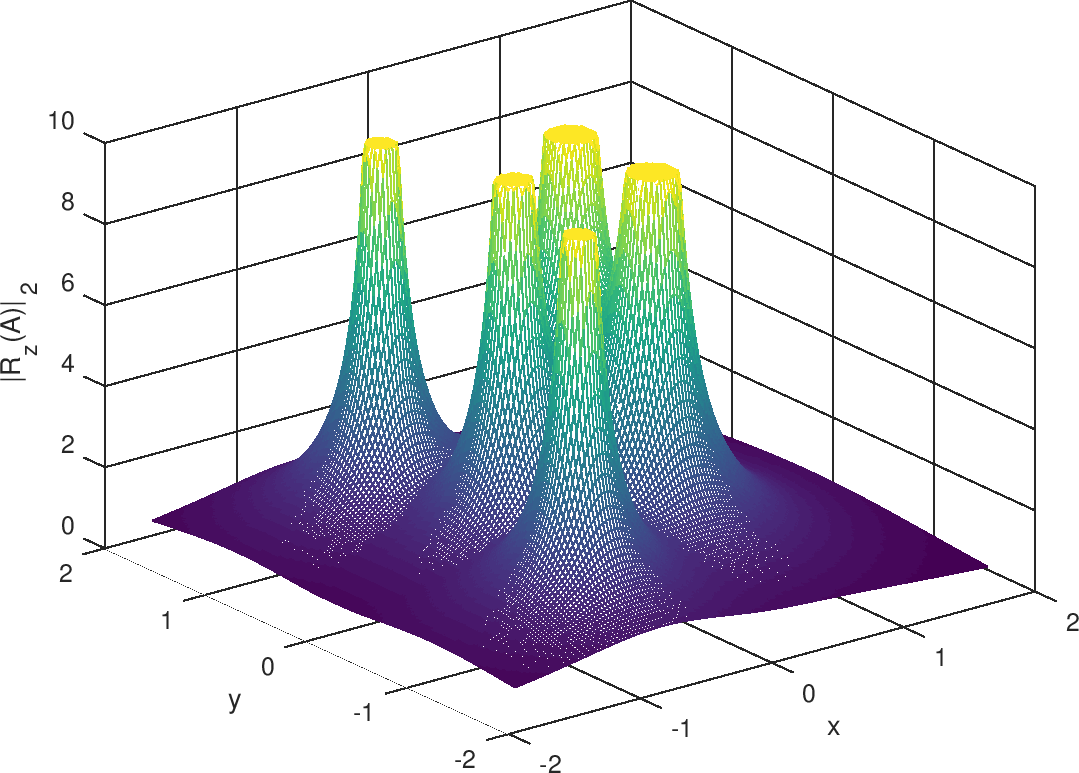
\includegraphics[width=0.45\textwidth]{figs/resolvesurf}
\end{itemize}
\end{frame}


\begin{frame}[fragile]
\frametitle{resolvent norms illustrated}

\begin{Verbatim}[fontsize=\footnotesize]
   >> [A,B] = gennormal(5);  % A,B have same eigs; A normal but B not
   >> resolveshow(A)         % normal case     (LEFT)
   >> resolveshow(B)         % nonnormal case  (RIGHT)
\end{Verbatim}

\bigskip
\begin{center}
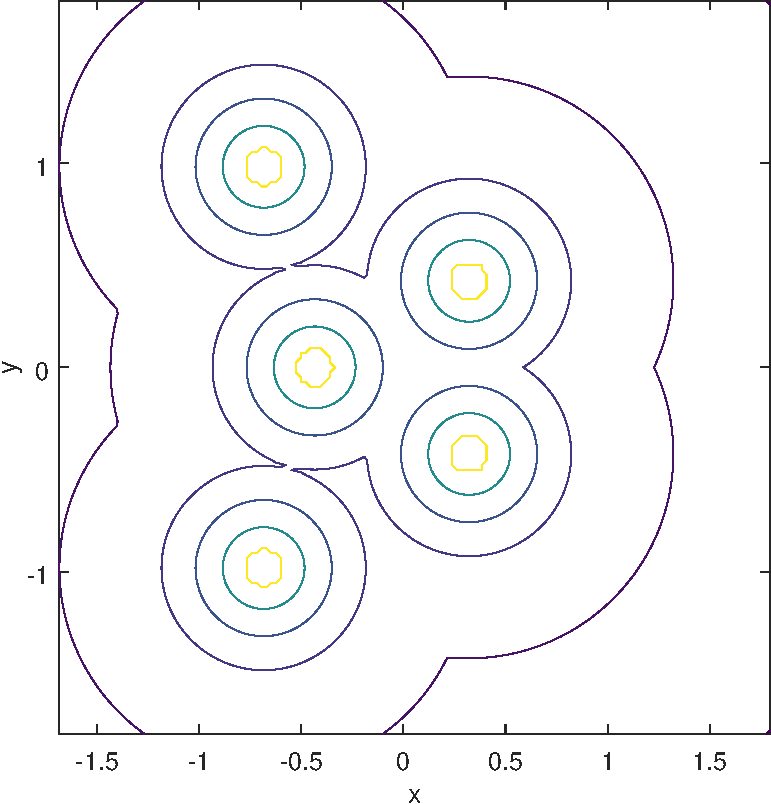
\includegraphics[width=0.31\textwidth]{figs/resolvenormal} \hspace{20mm} 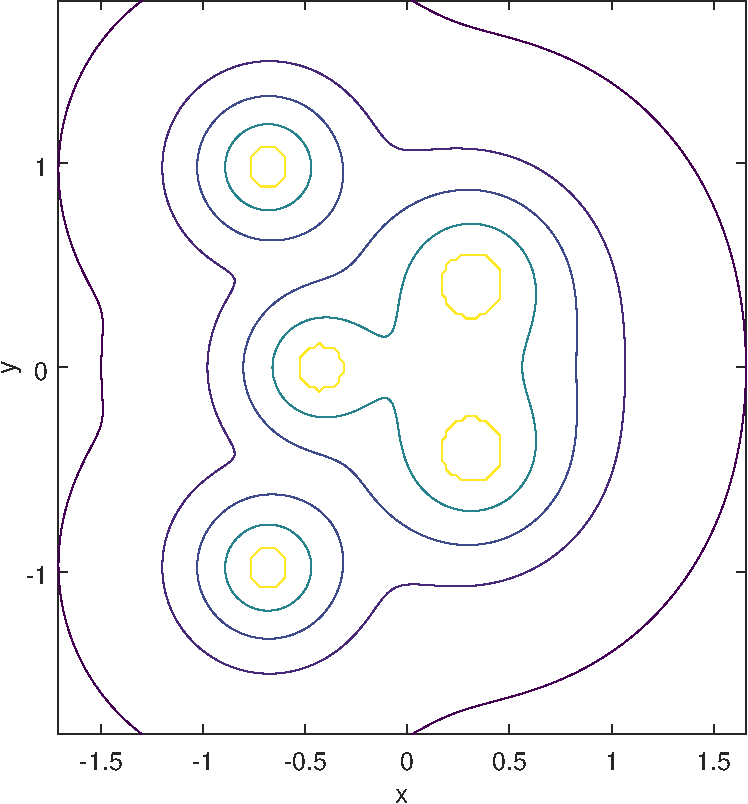
\includegraphics[width=0.3\textwidth]{figs/resolvenonnormal}
\end{center}

\small
\begin{itemize}
\item last slide already proved contours would be round for normal $A$
\item contours of $z\mapsto\|R_z(A)\|_2= \|(A-z I)^{-1}\|_2$ may be best spectral picture (personality test?) for nonnormal matrices $A$
    \begin{itemize}
    \item[$\circ$] $\sigma_\eps(A) = \left\{z\in\CC\,:\, \|(A-z I)^{-1}\|_2 \ge \eps^{-1}\right\}$ is the $\eps$-\emph{pseudospectrum} of $A$
    \end{itemize}
\end{itemize}
\end{frame}


\begin{frame}[fragile]
\frametitle{nonnormal matrices, a warning}

\begin{itemize}
\item facts and definitions:
    \begin{itemize}
    \item[$\circ$] $\|A^k\|\le \|A\|^k$ in any induced norm
    \item[$\circ$] if $A$ is normal then $\|A^k\|_2 = (\|A\|_2)^k = \rho(A)^k$
    \item[$\circ$] $\rho(A) = \max_{\lambda\in\sigma(A)} |\lambda|$
    \item[$\circ$] if $\rho(A)<1$ then $A^k \to 0$ as $k\to \infty$ \hfill \emph{proof?}
    \end{itemize}
\item but if $A$ is not normal and $\rho(A)<1$ then $\|A^k\|_2$ \emph{can be big} for a while
    \begin{itemize}
    \item[$\circ$] e.g.~random $100\times 100$ matrices $A$,$B$ with $\rho(A)=\rho(B)<1$
    \end{itemize}
\end{itemize}

\bigskip
\begin{Verbatim}[fontsize=\footnotesize]
   >> max(abs(eig(A)))
   ans =  0.90909
   >> max(abs(eig(B)))
   ans =  0.90909
\end{Verbatim}

\vspace{-17mm}
\hfill 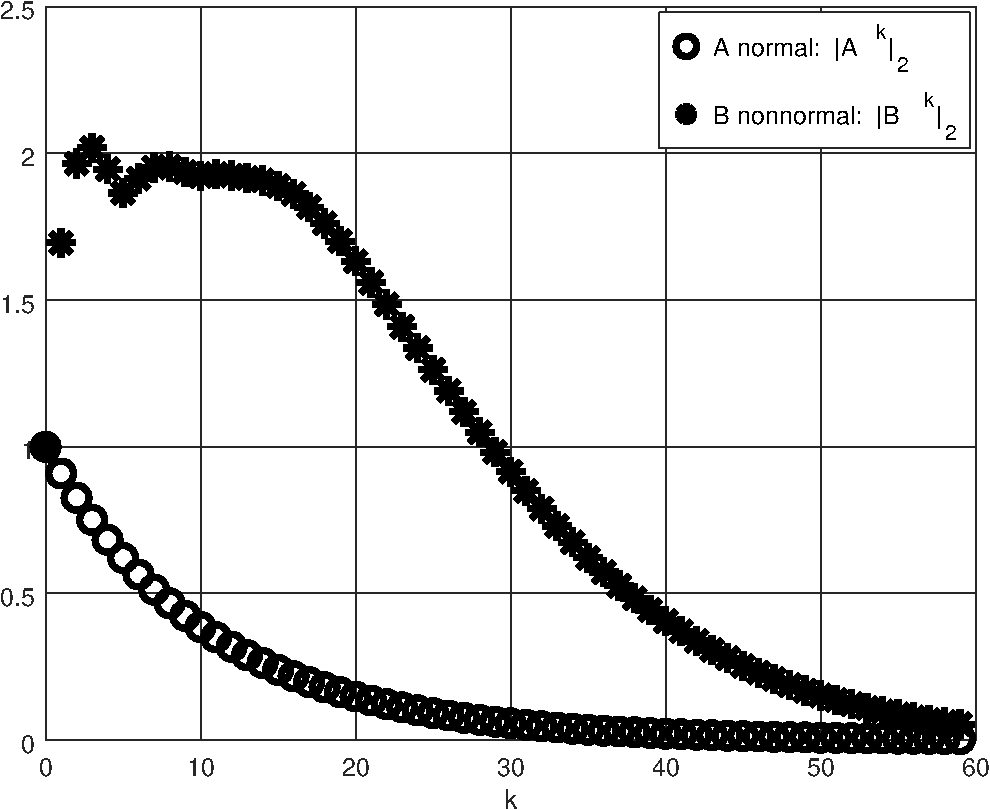
\includegraphics[width=0.45\textwidth]{figs/normpowers} \quad \phantom{foo}
\end{frame}


\section{orthogonal projections}

\begin{frame}{orthogonal projections}

\begin{definition}
$P \in \CC^{n\times n}$ is an \emph{orthogonal projection} if $P^2=P$ and $P^*=P$
\end{definition}

\begin{itemize}
\item if $\lambda \in \sigma(P)$ then $\lambda=0,1$
\item as for any projection ($P^2=P$):
    $$\ker P = \image (I-P), \quad \image P = \ker (I-P), \quad \CC^n = \ker P \oplus \image P$$
\item but now:
    $$\ker P \perp \image P$$

    \begin{itemize}
    \item[$\circ$] \emph{proof.}  if $u\in\ker P$ and $v=Pz\in\image P$ then $u^*v = u^*(Pz)=(Pu)^*z = 0$
    \end{itemize}
\item examples:
    $$0, \quad I, \quad P = \begin{bmatrix} 1 & & \\ & 1 & \\ & & 0 \end{bmatrix}$$
\end{itemize}
\end{frame}


\begin{frame}{constructing orthogonal projections}

\begin{itemize}
\item FIXME since hermitian, $P=Q \Lambda Q^* = \hat Q \hat Q^*$
\item e.g.~rank 1 case: $P=q q^*$
\item $P = A (A^* A)^{-1} A^*$
\end{itemize}
\end{frame}

\begin{frame}{x}

\begin{itemize}
\item y
\end{itemize}
\end{frame}

\begin{frame}[fragile]
\frametitle{X}

\begin{itemize}
\item FIXME  goal: a large normal matrix with spectrum mostly filling the unit circle

\begin{Verbatim}[fontsize=\scriptsize]
>> A0 = randn(100,100)/10;
>> [Q,R] = qr(randn(100,100));
>> norm(Q'*Q-eye(100))
ans =    1.8426e-15
>> [X,D] = eig(A0);
>> A = Q*D*Q';
>> norm(A'*A - A*A')
ans =    1.1396e-15
>> lam = eig(A);  plot(real(lam),imag(lam),'o')
>> grid on, axis equal
\end{Verbatim}

\end{itemize}
\end{frame}


\begin{frame}{resolution of the identity}

if $A$ normal then

$$Av = \sum_{i=1}^n \lambda_i q_i (q_i^*v)$$

$$A = \sum_{i=1}^n \lambda_i q_i q_i^*$$

\footnotesize
\href{https://en.wikipedia.org/wiki/Spectral_theory\#Resolution_of_the_identity}{\texttt{en.wikipedia.org/wiki/Spectral\_theory\#Resolution\_of\_the\_identity}}
\end{frame}


\section{singular value decomposition}

\begin{frame}{x}

\begin{itemize}
\item y
\end{itemize}
\end{frame}

\end{document}
